\documentclass[]{article}

\usepackage[english]{babel}
\usepackage[utf8x]{inputenc}
\usepackage[T1]{fontenc}
 
\usepackage[a4paper,margin=2 cm]{geometry}
 
%% Useful packages
\usepackage{amsmath}
\usepackage{graphicx}
\usepackage{para list}
\usepackage{indentfirst}
\usepackage{booktabs}
\usepackage{multirow}
\usepackage{clrscode}
\usepackage{listings}
\usepackage{multicol}
\usepackage{graphicx}

\begin{document}
\begin{multicols*}{2}
\title{ASR EXPERIMENTS}
\author{Tom}
\maketitle

\section{Introduction}

\section{Monophone Model}
\subsection{Number of Gaussian}
\subsubsection{Purpose}
The aim of this task is to investigate how the number of Gaussian mixture components influences WER, and find the optimal number that gives the lowest WER. 

\subsubsection{Implementation}
We want to test the model with different number of Gaussian mixture components. So, we modify the parameter of $train\_mono.sh$ script.

\begin{lstlisting}[language=sh,showstringspaces=false,numbers=left,tabsize=4, xleftmargin=\parindent, frame=single, basicstyle=\tiny] 
# we previously set a parameter $num_gauss to
# store the number of gaussian 
steps/train_mono.sh --nj 4 --totgauss $num_gauss \
	data/train data/lang exp/mono

\end{lstlisting}

To evaluate the time consuming, we also compute the the time used in the process of training model and decoding.

\begin{lstlisting}[language=sh,showstringspaces=false,numbers=left,tabsize=4, xleftmargin=\parindent, frame=single, basicstyle=\tiny] 
# store start time
start_time=$(date +%s)

# code to train model and decode
......

# store end time
end_time=$(date +%s)

# compute runing time
echo "runing time" $(($end_time - $start_time))

\end{lstlisting}


\subsubsection{Experiments and Results}
We start with setting a large range for the number of Gaussian mixture components (n), starting from 500  and going till 20000 with the step of 250. The results of the experiment in terms of WER and time are shown in Figure 1.1.1 and Figure 1.1.2 respectively.

\begin{center}
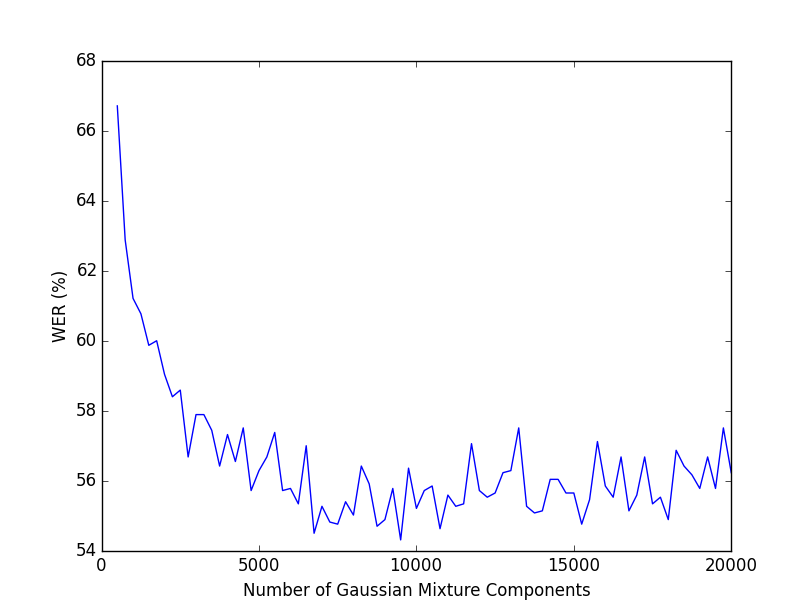
\includegraphics[width=3in]{figure_1_WER.png} 
Figure 1.1.1: WER against number of Gaussian mixture components (500<n<20000).
\end{center}

\begin{center}
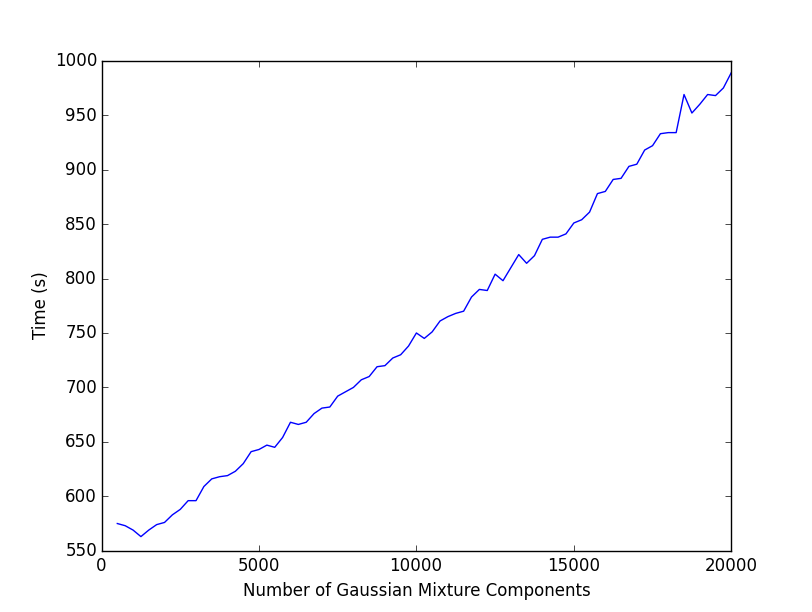
\includegraphics[width=3in]{figure_1.png} 
Figure 1.1.2: Time against number of Gaussian mixture components (500<n<20000).
\end{center}

As we can see from Figure 1.1.2, the time consuming increases linearly with the increase of the number of gaussian mixture components.  According to Figure 1.1.1, WER generally decreases with the increase of Gaussian mixture components when n<10000. After that, WER tends to convergence, fluctuating between 54\% and 58\%. The lowest WER occurs around n=9500, so we focus on the range (9500,9800) to run our script again in order to see if we could generate a better result in that range. Figure 1.1.3 shows the result of further experiment.
\begin{center}
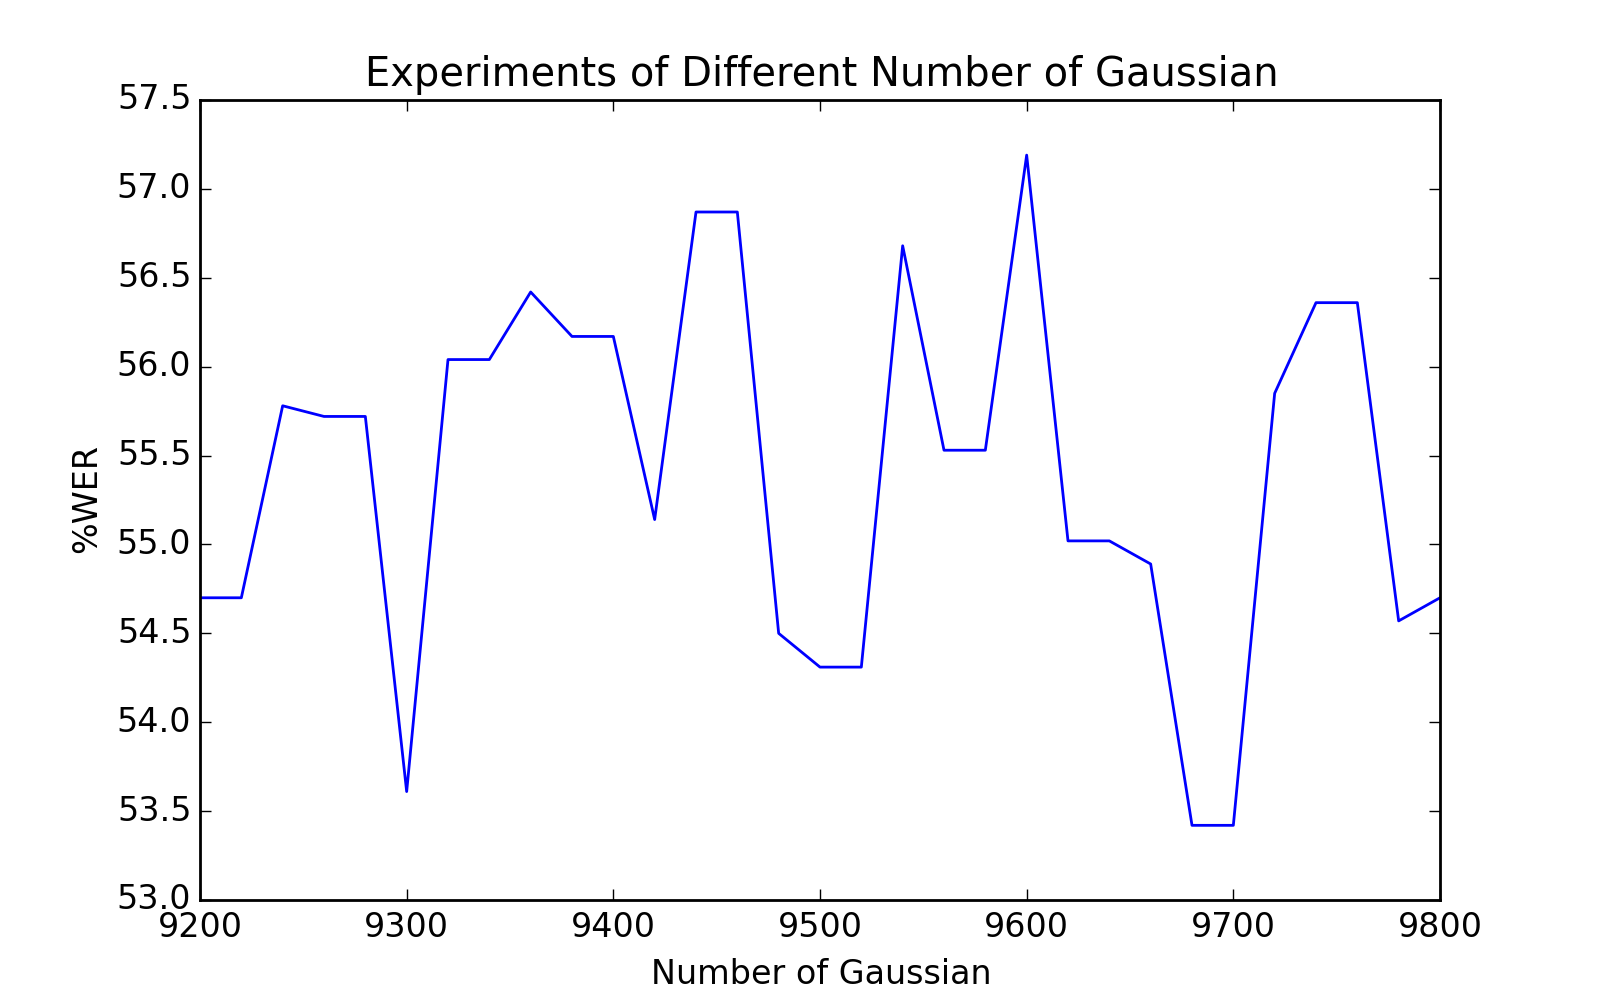
\includegraphics[width=3in]{result1_detailed_wer_new.png} 
Figure 1.1.3: WER against number of gaussian mixture components (9500<n<9800).
\end{center}
Form the plot, we find that the lowest WER we obtained is 53.42\%  , where the number of gaussian mixture components is about 9700.

\subsubsection{Conclusion and Discussion}
From the results we got in experiments, we could investigate that with the increase of the number of gaussian mixture components, the WER decreases on the whole. When the number of gaussian is less than 3000, the WER decreases smoothly. After that, the evolution of WER starts fluctuating but still has the trend of decreasing. Until the number of gaussian mixture components reaches around 7000, the WER fluctuates in a small range. So, to sum up, the WER will finally converge with the increase of number of gaussian mixture components.

To briefly explain this, we refer to Mark's review work. We think if we give a large number of gaussian, the gaussians used to express the distribution of state transformation of each phone increases so that the distribution is characterized very precise. This is the reason why a higher gaussian will lead to a better recognition result. Meanwhile, too much gaussian will also cause some problem because the extra components will cause noise as well. This explains the cause of fluctuating parts of the evolution plot.

As for the time consuming, we could easily come to this conclusion that the time consuming has a perfect linear relationship with the number of gaussian mixture components. So, to search the best model, we could try small gaussians to save time.

The best model we obtained is shown in script run\_mono\_t1\_best.sh (where the number of gaussian mixture components is 9700).

\subsection{Features}
\subsubsection{Purpose}
The aim of this part is to use MFCC, PLP and Filter bank with the optimal number of Gaussian mixture components(9700) obtained in task 1.1 to investigate how different acoustic features give different WERs. 

\subsubsection{Implementation}
To extract different kinds of features(mfcc, plp and fbank), we write a loop in script to obtain different features.

\begin{lstlisting}[language=sh,showstringspaces=false,numbers=left,tabsize=4, xleftmargin=\parindent, frame=single, basicstyle=\tiny] 
for feats in mfcc plp fbank; do
	for dir in train test; do
		# extract features
		steps/make_$feats.sh data/$dir /
			exp/make_$feats/$dir $feats
		# compute cmvn
		steps/compute_cmvn_stats.sh data/$dir /
			exp/cmvn/$dir cmvn
	done	
	# code to train model and decode
	......
done

\end{lstlisting}

\subsubsection{Experiments and Result}
Figure 1.2.1 and Figure 1.2.2 respectively show the comparisons among the three acoustic features in terms of WER and time.

\begin{center}
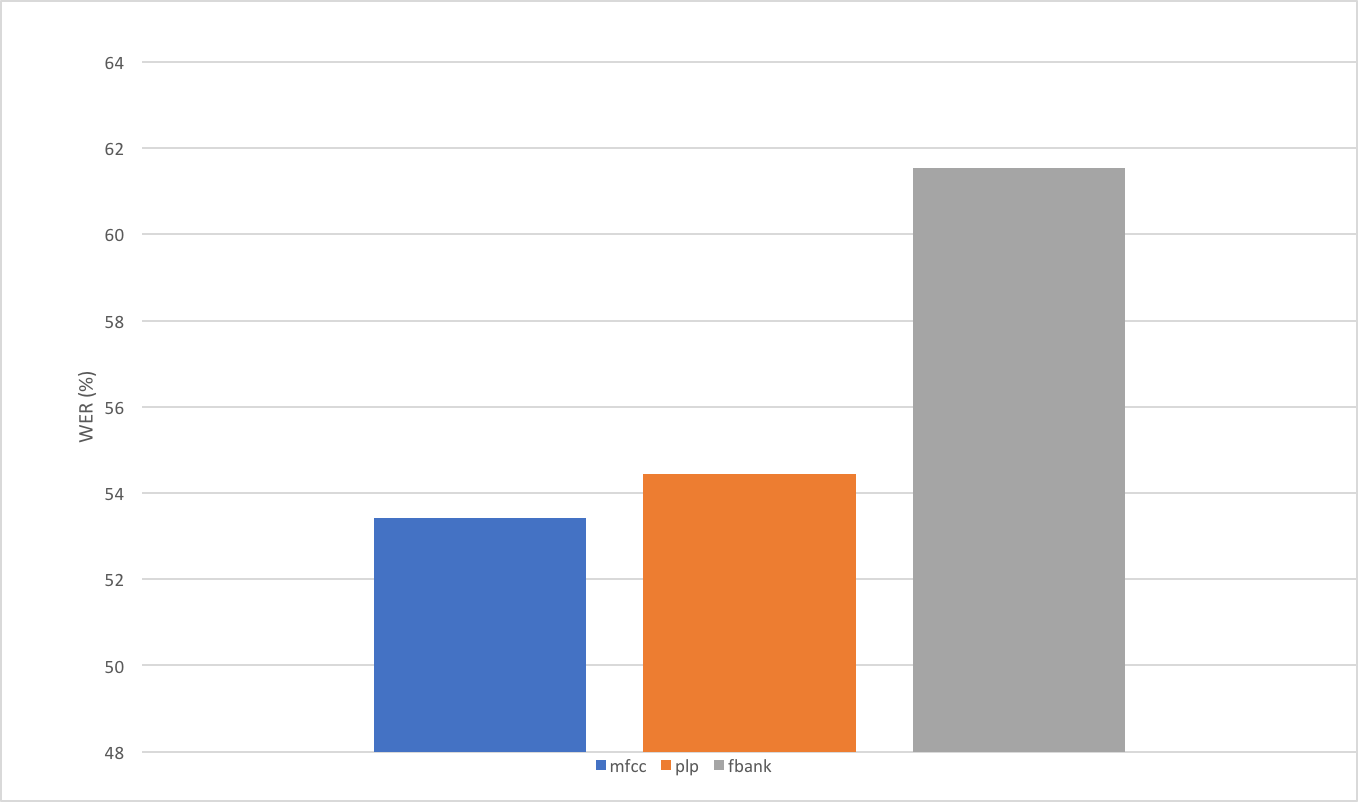
\includegraphics[width=3in]{Picture2.png} 
Figure 1.2.1: WERs of different acoustic features.
\end{center}

\begin{center}
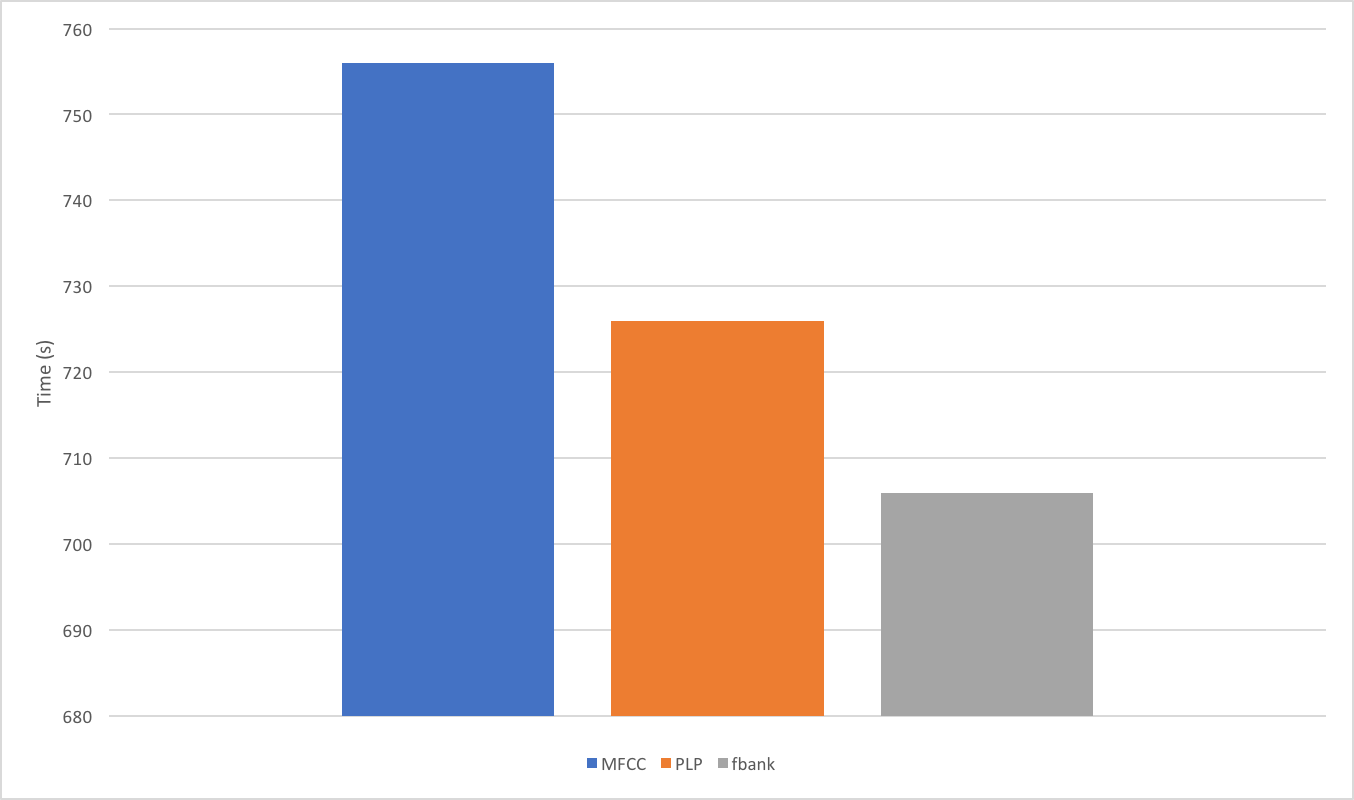
\includegraphics[width=3in]{Picture1.png} 
Figure 1.2.2: Time of different acoustic features.
\end{center}

WERs of MFCC, PLP and Fbank are 53.42\%, 54.44\% and 61.53\% respectively. Time of MFCC, PLP and Fbank are 756s, 726s and 702s respectively. MFCC has the lowest WER while the WER of Fbank is much higher than that of MFCC and PLP. However, Fbank takes the shortest time, PLP is the second and MFCC needs the longest time.

\subsubsection{Conclusion and Discussion}

MFCCs are based on the log spectral envelope of the speech signal, transformed to a nonlinear frequency scale that roughly corresponds to that observed in the human auditory system.This kind of feature is widely used in standard HMM-GMM model. However, it's not robust against noise.

Perceptual linear prediction(PLP) feature uses linear predictive auto-regressive modelling to obtain cepstral coefficients. it is a frequently used alternative acoustic feature analysis, which  includes an auditory-inspired cube-root compression and uses an all-pole model to smooth the spectrum before the cepstral coefficients are computed (Hermansky, 1990). And it is better noise robustness.

As for Fbanks, it is a part of MFCCs features and is widely used in DNN ASR model.

As what is shown in the plot, MFCCs and PLP could obtain similar results and Fbank gives the worst result though it costs less time. Therefore, in conclusion, MFCCs and PLP are very good features in automatic speech recognition task.

So, what advantages do MFCCs and PLP have? A particular advantage of cepstral representations compared with spectral representations is the decorrelation of cepstral  coefficients,  compared  with  the  high  correlations  observed  between neighbouring spectral coefficients(R\&H review, 2010). Such decorrelations are very well matched with the distributional assumptions that underlie systems based on Gaussians with diagonal covariance matrices.

\subsection{Dynamic Features}
\subsubsection{Purpose}
The aim of this task is to investigate how the dynamic features (i.e. delta and delta delta features) of MFCCs influence WER. To generate comparable result, we set the $--use-energy$ to false for all MFCCs in this experiment.

\subsubsection{Implementation}
The scripts use the pipeline to generate the dynamic features of the extracted features. 

The original code of generating features is:

\begin{lstlisting}[language=sh,showstringspaces=false,numbers=left, title=\lstname{Creating dynamic feature with pipeline method},tabsize=4, xleftmargin=\parindent, basicstyle=\tiny, frame=single] 
feats="ark,s,cs:apply-cmvn $cmvn_opts \
	--utt2spk=ark:$sdata/JOB/utt2spk \
	scp:$sdata/JOB/cmvn.scp \
	scp:$sdata/JOB/feats.scp ark:- | \ 
	add-deltas $delta_opts ark:- ark:- |";;
\end{lstlisting} 

We find that the dynamic features(delta and delta-delta features) are generated in third line with $add-delta$ command. So, we delete this part for not creating dynamic features. New code is shown below:

\begin{lstlisting}[language=sh,showstringspaces=false,numbers=left, tabsize=4, xleftmargin=\parindent, basicstyle=\tiny, frame=single] 
feats="ark,s,cs:apply-cmvn $cmvn_opts \
	--utt2spk=ark:$sdata/JOB/utt2spk \
	scp:$sdata/JOB/cmvn.scp \
	scp:$sdata/JOB/feats.scp ark:- |";;
\end{lstlisting} 

To obtain delta feature, we could simple option $--delta-order=1$ in $add-delta$ command. 

To check the new features without dynamic feature, we display the dimension of new features by using below command:

\begin{lstlisting}[language=sh,showstringspaces=false,numbers=left,tabsize=4, xleftmargin=\parindent, frame=single, basicstyle=\tiny] 
apply-cmvn --utt2spk=ark:data/train/utt2spk \ 
	scp:data/train/cmvn.scp \
	scp:data/train/feats.scp ark:- | \
	feat-to-dim ark:- -
	
# output:
13
\end{lstlisting}


\subsubsection{Experiment}
We set the number of Gaussian mixture components to be 9700. Since the sample scripts used in the labs employ dynamic features, we copied train\_mono.sh and decode.sh to my-local and deleted the delta features in the codes. The original method using delta and delta-delta features obtains a WER of 53.42\%. The method using only delta feature obtains a WER of 60.51\% while the method using no dynamic feature obtains a WER of 81.34\%. The results of this experiment is shown in Figure 1.3.1 and Figure 1.3.2. 

\begin{center}
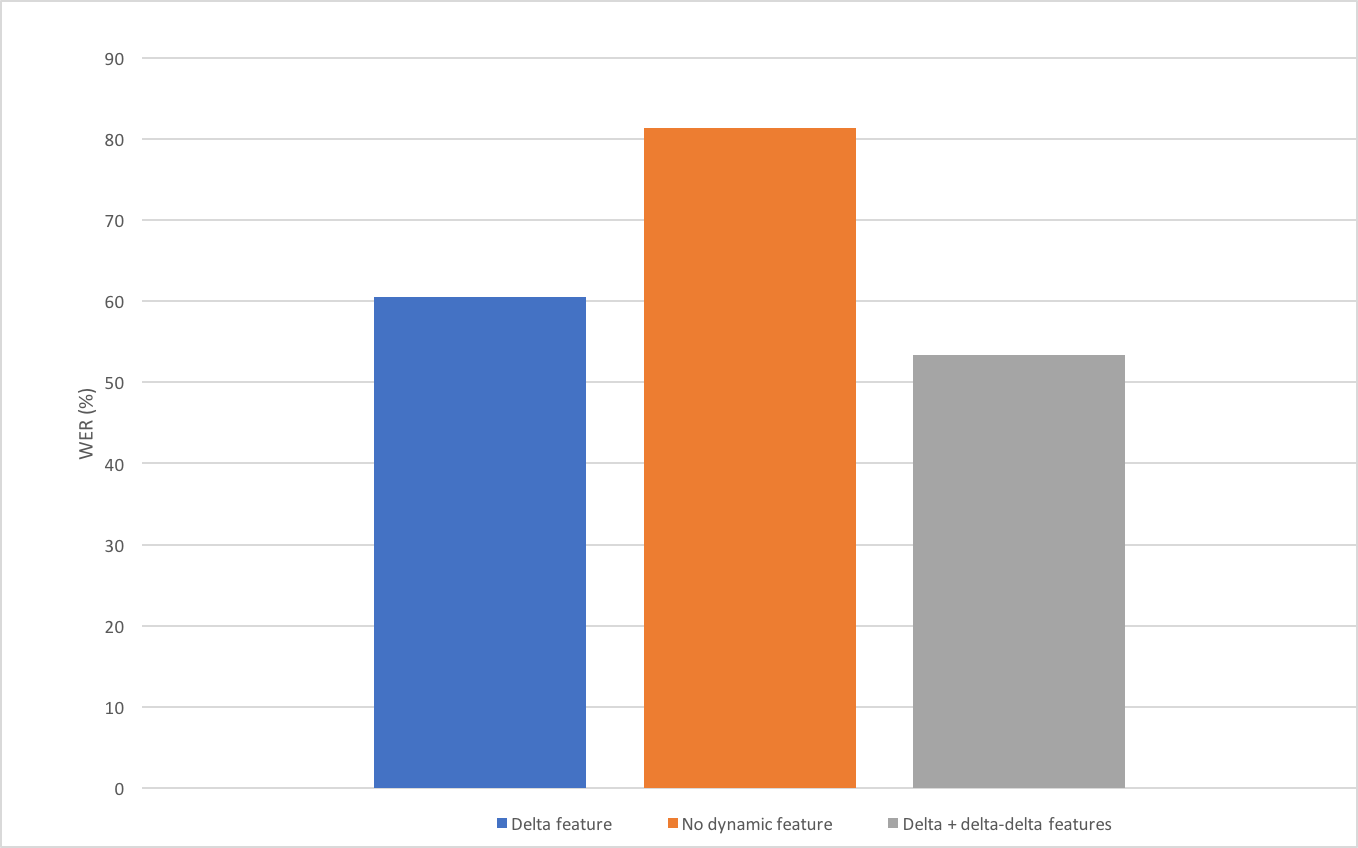
\includegraphics[width=3in]{Picture4.png} 
Figure 1.3.1: WERs of using and not using dynamic features.
\end{center}

\begin{center}
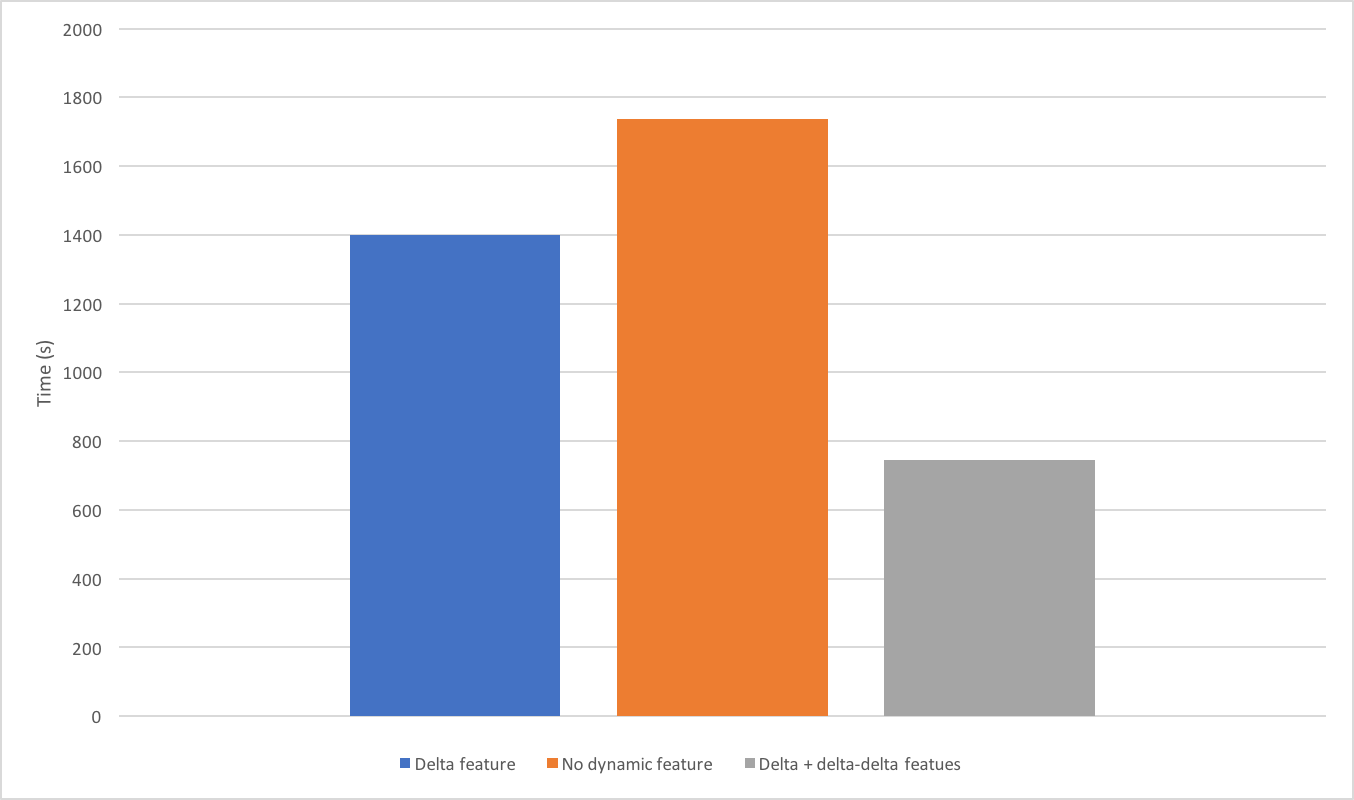
\includegraphics[width=3in]{Picture3.png} 
Figure 1.3.2: Time of using and not using dynamic features.
\end{center}

We can see that using delta feature and delta-delta feature (dynamic features) can much decrease the WER and time.

\subsubsection{Conclusion and Discussion}
From the experiment results, we could find that dynamic feature significantly improves the recognition result. The dynamic feature is generated by adding features to do with how the cepstral coefficients change over time. Speech recognition accuracy is substantially improved if the feature vectors are augmented with the first and second temporal derivatives of the acoustic features (sometimes referred to as the deltas and delta-deltas), thus adding some information about the local temporal dynamics of the speech signal to the feature representation (Furui, 1986)

Adding such temporal information to the acoustic feature vector introduces a direct dependence between successive feature vectors, which is not usually taken account of in acoustic modelling; a mathematically correct treatment of these dependences has an impact on how the acoustic model is normalized—since fewer feature vector sequences will be consistent—and results in an approach we may be viewed as modelling an entire trajectory of feature vectors.

\subsection{CMN/CVN}
\subsubsection{Purpose}
The aim of this task is to investigate the influence of CMVN on WER. In the sample scripts, CMVN is used. So, we avoided using CMVN in the experiment.
\subsubsection{Implementation}
We find that there is a parameter in $compute\_cmvn\_stats.sh$ that could help to create the features without CMVN, which is the $fake$ option. So, we modify the extracting feature part like this.
\begin{lstlisting}[language=sh,showstringspaces=false,numbers=left,tabsize=4, xleftmargin=\parindent, frame=single, basicstyle=\tiny] 
for dir in train test; do
	# extract features
	steps/make_mfcc.sh data/$dir /
		exp/make_mfcc/$dir mfcc
	# compute fake cmvn
	steps/compute_cmvn_stats.sh --fake data/$dir /
		exp/cmvn/$dir cmvn
\end{lstlisting}

\subsubsection{Experiment}
We set the number of Gaussian mixture components to be 9700. The WER we got without using CMVN is 58.40\%, higher than 53.42\% (using CMVN). However, the time of using no CMVN is 736s whcih is 20s  shorter than that of using CMVN.


\section{Triphone Model}
\subsection{Aim}
The aim of this task is to investigate the influences of the number of clusters and the number of Gaussian mixture components on WER and seek a optimal com- bination that gives the lowest WER.
\subsection{Implementation}
This time, we want to investigate two parameters of $train\_deltas.sh$ script in exponential range. So, the experiment script is modified like this.
\begin{lstlisting}[language=sh,showstringspaces=false,numbers=left,tabsize=4, xleftmargin=\parindent, frame=single, basicstyle=\tiny] 
for ((num_cluster=1000;num_cluster<=4000; \
	num_cluster=um_cluster+1000)); do
	for ((per_gauss=1;per_gauss<=64; \
		per_gauss=per_gauss*2)); do
		# code to train model and decode
		......
	done
done
\end{lstlisting}

\subsection{Experiment}
We set the number of clusters to start from 1000 to 5000, in steps of 500. The number of Gaussian mixture components is equal to the number of clusters multiply $2^n$ (n=0, 1, 2, 3, 4, 5). The results are shown in Figure 2.

\begin{center}

\end{center}

\section{Adaptive Training}
\subsection{Gender Dependent System}
\subsubsection{Aim}
The aim of this task is to develop gender dependent acoustic models and make the recognition.
\subsubsection{Implementation}
To train a gender dependent model, we manually split the data into two part: female subset and male subset. We implement this by writing a python file to split the original data file.

\subsubsection{Experiment}
\begin{center}
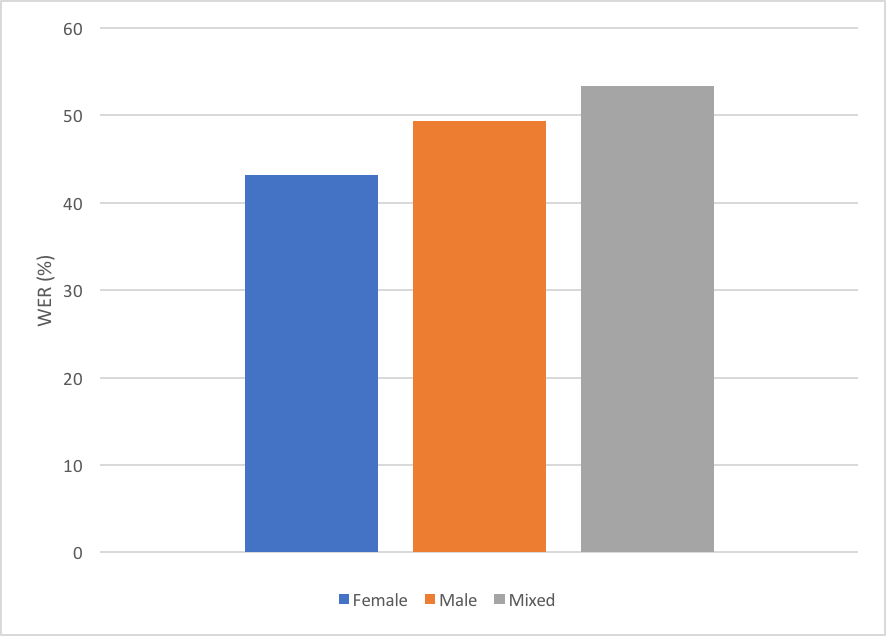
\includegraphics[width=3in]{Picture5.png} 
Figure 3: WER of gender dependent acoustic model and original model.
\end{center}

We can see the gender dependent acoustic model improves the WER. The WER of female acoustic  recognition is 43.13\% and the WER of male acoustic recognition is 49.38\%, both lower than the WER of the original one.

\subsection{Feature Transformation and Adaptive Training}
\subsubsection{Vtln Feature}
\subsubsection{fMLLR}

\end{multicols*}
\end{document}